% File: 8BallPool video analysis
\documentclass[letterpaper,12pt]{article} % DO NOT CHANGE THIS

\usepackage{amsmath}
\usepackage{amsfonts}

%\usepackage{aaai24}  % DO NOT CHANGE THIS
\usepackage{times}  % DO NOT CHANGE THIS
\usepackage{helvet}  % DO NOT CHANGE THIS
\usepackage{courier}  % DO NOT CHANGE THIS
\usepackage[hyphens]{url}  % DO NOT CHANGE THIS
\usepackage{graphicx} % DO NOT CHANGE THIS
\urlstyle{rm} % DO NOT CHANGE THIS
\def\UrlFont{\rm}  % DO NOT CHANGE THIS
\usepackage{natbib}  % DO NOT CHANGE THIS AND DO NOT ADD ANY OPTIONS TO IT
\usepackage{caption} % DO NOT CHANGE THIS AND DO NOT ADD ANY OPTIONS TO IT
\usepackage{subcaption}
\frenchspacing  % DO NOT CHANGE THIS
\setlength{\pdfpagewidth}{8.5in}  % DO NOT CHANGE THIS
\setlength{\pdfpageheight}{11in}  % DO NOT CHANGE THIS
\usepackage{array}
%
% These are recommended to typeset algorithms but not required. See the subsubsection on algorithms. Remove them if you don't have algorithms in your paper.
\usepackage{algorithm}
\usepackage{algorithmic}
\usepackage{fullpage}

%
% These are are recommended to typeset listings but not required. See the subsubsection on listing. Remove this block if you don't have listings in your paper.
\usepackage{newfloat}
\usepackage{listings}
\DeclareCaptionStyle{ruled}{labelfont=normalfont,labelsep=colon,strut=off} % DO NOT CHANGE THIS
\lstset{%
	basicstyle={\footnotesize\ttfamily},% footnotesize acceptable for monospace
	numbers=left,numberstyle=\footnotesize,xleftmargin=2em,% show line numbers, remove this entire line if you don't want the numbers.
	aboveskip=0pt,belowskip=0pt,%
	showstringspaces=false,tabsize=2,breaklines=true}
\floatstyle{ruled}
\newfloat{listing}{tb}{lst}{}
\floatname{listing}{Listing}
%
% Keep the \pdfinfo as shown here. There's no need
% for you to add the /Title and /Author tags.
\pdfinfo{
/TemplateVersion (2024.1)
}

% DISALLOWED PACKAGES
% \usepackage{authblk} -- This package is specifically forbidden
% \usepackage{balance} -- This package is specifically forbidden
% \usepackage{color (if used in text)
% \usepackage{CJK} -- This package is specifically forbidden
% \usepackage{float} -- This package is specifically forbidden
% \usepackage{flushend} -- This package is specifically forbidden
% \usepackage{fontenc} -- This package is specifically forbidden
% \usepackage{fullpage} -- This package is specifically forbidden
% \usepackage{geometry} -- This package is specifically forbidden
% \usepackage{grffile} -- This package is specifically forbidden
% \usepackage{hyperref} -- This package is specifically forbidden
% \usepackage{navigator} -- This package is specifically forbidden
% (or any other package that embeds links such as navigator or hyperref)
% \indentfirst} -- This package is specifically forbidden
% \layout} -- This package is specifically forbidden
% \multicol} -- This package is specifically forbidden
% \nameref} -- This package is specifically forbidden
% \usepackage{savetrees} -- This package is specifically forbidden
% \usepackage{setspace} -- This package is specifically forbidden
% \usepackage{stfloats} -- This package is specifically forbidden
% \usepackage{tabu} -- This package is specifically forbidden
% \usepackage{titlesec} -- This package is specifically forbidden
% \usepackage{tocbibind} -- This package is specifically forbidden
% \usepackage{ulem} -- This package is specifically forbidden
% \usepackage{wrapfig} -- This package is specifically forbidden
% DISALLOWED COMMANDS
% \nocopyright -- Your paper will not be published if you use this command
% \addtolength -- This command may not be used
% \balance -- This command may not be used
% \baselinestretch -- Your paper will not be published if you use this command
% \clearpage -- No page breaks of any kind may be used for the final version of your paper
% \columnsep -- This command may not be used
% \newpage -- No page breaks of any kind may be used for the final version of your paper
% \pagebreak -- No page breaks of any kind may be used for the final version of your paper
% \pagestyle -- This command may not be used
% \tiny -- This is not an acceptable font size.
% \vspace{- -- No negative value may be used in proximity of a caption, figure, table, section, subsection, subsubsection, or reference
% \vskip{- -- No negative value may be used to alter spacing above or below a caption, figure, table, section, subsection, subsubsection, or reference

\usepackage{enumitem}
\usepackage{nameref}
\usepackage{adjustbox}
\graphicspath{{./img/}}


\setcounter{secnumdepth}{0} %May be changed to 1 or 2 if section numbers are desired.

% The file aaai24.sty is the style file for AAAI Press
% proceedings, working notes, and technical reports.

% Title

% Your title must be in mixed case, not sentence case.
% That means all verbs (including short verbs like be, is, using,and go),
% nouns, adverbs, adjectives should be capitalized, including both words in hyphenated terms, while
% articles, conjunctions, and prepositions are lower case unless they
% directly follow a colon or long dash
\title{8BallPool video analysis}
\author{
	%Authors
	Michele Sprocatti\textsuperscript{\rm 1}, %\equalcontrib,
	Alberto Pasqualetto\textsuperscript{\rm 2}, %\equalcontrib,
	Michela Schibuola\textsuperscript{\rm 3}\\
}

\begin{document}
%\nocopyright
\maketitle

\begin{center}
	Department of Information Engineering, University of Padua\\
	Via Gradenigo 6, 35131 Padova, Italy\\
	% email address must be in roman text type, not monospace or sans serif
	% proceedings-questions@aaai.org
	\{michele.sprocatti\textsuperscript{\rm 1}, alberto.pasqualetto.2\textsuperscript{\rm 2}, michela.schibuola\textsuperscript{\rm 3}\}@studenti.unipd.it
\end{center}

% TODO write about restrictions in the input datasets size/aspect ratio

\section{Introduction}

This is the report of the final project for the Computer Vision course, which goal is to develop a computer vision system for analyzing video footage of various “Eight Ball” billiard game events.

\section{How the work has been split}
The three group members collaborated by dividing the work. Each member was responsible for producing specific files, all of which were annotated with their respective author.

\subsection{Split of the work}
The source code reflects a division of labor across three key areas:
\begin{enumerate}
	\item Detection and segmentation of balls and the playing table: this area, along with the main program functionality, was handled by Michele.
	\item Metrics calculation and tracking: responsibility for this area fell to Alberto.
	\item Transformation code and mini-map management: this area was overseen by Michela.
\end{enumerate}

\subsection{Working hour per member}
The approximate number of working hours for each member of the group are:
\begin{description}
	\item[Michele:] 50 hours
	\item[Michela:] 50 hours
	\item[Alberto:] 50 hours
\end{description}
% TODO hours


\section{Elements of our project}

\section{Executables}
The program contains 4 different executables:
\begin{itemize}
	\item \texttt{8BallPool}: the main executable that, given a video file, it processes it and creates the output video with the superimposed minimap.
	\item \texttt{TestAllClip}: it is the executable used to test the detection and segmentation in the first and last frame of all videos through AP and IoU by comparing them with the ground truth.
	\item \texttt{ShowSegmentationColored}: is an helper which has been used to show the ground truth of the segmentation of a particular frame using human-readable colors and it was also used as a test for the code that computes the metrics because it computes the performance of the ground truth on itself.
	\item \texttt{ComputePerformance}: is used to compute the performance across the dataset so the mAP and the mIoU.
\end{itemize}

% TODO cmd parameters

\subsection{Table detection}
A mask-based approach was implemented for table detection, exploiting the fact that in billiard game footage, the table should be always located in the middle of the frame; this assumption is confirmed by all the videos in the dataset.
The mask was generated by identifying the most common color in the image's central columns; the color is represented by a range in the Hue component (with respect to HSV color space).
Building upon this initial step, Michele exploits the Canny edge detector and OpenCV's HoughLinesP function.
Then the function analyzes the found intersections and merges nearby points, ensuring the consistent identification of 4 corner points corresponding to the table's corners in the processed dataset.

\subsection{Table segmentation}

In order to isolate the table with high precision, Michele employed a combination on two different binary masks through a voting system.
The involved masks are:
\begin{description}
	\item[Color-based mask] Created by identifying pixels corresponding to the table's color range. This mask is very robust on shadows and reflections since it defined through the Hue component of the HSV color space, which is invariant to brightness.
	\item[k-means clustering mask] Generated by applying the k-means algorithm on the image to separate the table from the background. Useful when the table color range is too broad to be captured by the color-based mask.
\end{description}
These two masks are combined through a voting system, which classifies as table pixels classified as such by at least one of the two masks gaining the best of both approaches.
Finally the isolated area is limited to the pixels inside the polygon defined by the previously detected corners.

\subsection{Balls detection}
To detect balls, Michele proposed a multi-step preprocessing approach. Initially, the table region is isolated using an approach similar to the segmentation described before. Then the corners area is removed to prevent Hough Circle transform to find them as false positives. Subsequently k-means clustering was applied to the image with k=5 (the number of balls type plus the playing field). The resulting clusterized \texttt{Mat} is converted to gray-scale to be used as \texttt{HoughCircle} input. The gray-scale output colors were selected to be as different from each other once the color space is changed.

Circle parameters, such as radius and center color, were analyzed to identify potential ball regions. By calculating the mean radius of in-table circles with center not selected by the color mask, a radius range was established. Circles within this radius range were considered for further analysis.

Ball classification involved creating a circular mask, computing the gray-scale histogram, and excluding background pixels from the values of the histogram. Peak values in the histogram were used to differentiate between striped and solid balls, while HSV color space analysis is used to distinguish white and black balls.

After finding the balls, the team identified an optimization opportunity. Since there's only one white ball and one black ball, Michele implemented non-maxima suppression for white and black balls independently, in order to improve performance.

The result of the detection process is then used to segment the balls.

\subsubsection{Attempt of ball radius relative to the distance and perspective of the camera with respect to the table}

To try to increase the performance of the ball detection, it has been attempted to compute an interval of values for the ball radius relative to the pixels of the image and the position of the camera with respect to the table; this would have been used in the \texttt{HoughCircles()}. For that purpose, the \texttt{radiusInterval()} method has been written. This method starts by computing the mean radius value by using a proportion between the diagonal of the table in pixels and the approximate dimensions of the diagonal of the table and the balls in centimeters. 
\begin{equation}
	mean\_radius =  \frac{ball\_radius\_cm}{table\_diagonal\_cm} longest\_diagonal\_px
\end{equation}
Then, a percentage of the slope between the camera direction and the table has been computed, by using one of the angles (<90°) that the detected table creates; this angle is compared with the PI/2 angle, and a value between 0 and 1 is computed:

\begin{equation}
	percentage\_slope = 1 - \frac{minimum\_angle}{\pi}
\end{equation}

\begin{itemize}
	\item If the value is 1, then the camera is parallel to the table;
	\item If the value is 0, then the camera is perpendicular to it;
	\item If, for example, the value is 0.5, then the camera is about 45° from the table.
\end{itemize}
	
To compute the final interval, the minimum and maximum values are computed by subtracting and incrementing a value, which increases with the percentage of slope (more the slope, more the variance) by multiplying the percentage of slope with the mean radius previously computed, and a precision value is added due to some other variables in the images.
\begin{equation}
	half\_interval = mean\_radius*percentage\_slope + prec
\end{equation}
\begin{equation}
	min\_radius = mean\_radius - half\_interval
\end{equation}
\begin{equation}
	max\_radius = mean\_radius + half\_interval
\end{equation}

\
The idea of trying this method was from Michela.

\subsection{Tracking}
\subsection{Minimap creation}
To create the minimap are needed:
\begin{itemize}
	\item An image that contains an empty billiard table and some information about it;
	\item The position of the balls in the current and previous frames;
	\item A transformation matrix that computes the position of the balls in the minimap.
\end{itemize}

\subsubsection{Empty minimap image}
As a first step, an image of an empty billiard table has been selected, and its corner positions and dimensions have been stored in constant variables by testing different values. In particular, Alberto had the idea of converting the image into a byte array and inserting it in a header file through ImageMagick (\url{https://imagemagick.org/}).
This step has been performed with the aim of creating a self-contained executable without the need for the \texttt{.png} image dependency.
The byte array is then used to create a \texttt{Mat} object through the \texttt{imdecode} function.

\subsubsection{Computation of the transformation matrix}
The \texttt{computeTransformation} method has been written to compute the transformation matrix, which allows for the computation of the positions of the balls in the 2d table represented in the minimap. To do that, a relationship between the corners of the table in the frame and the corners of the table in the minimap has been found by the OpenCV \texttt{getPerspectiveTransform()} method, which “calculates a perspective transform from 4 pairs of the corresponding points” and returns a transformation matrix.
At first, it is supposed that the corners are given in clockwise order and that the first corner is followed by a long table edge. To check this information, \texttt{checkHorizontalTable} has been written.

\subsubsection{Check if the corners are in the required order}
The \texttt{checkHorizontalTable} method checks, using the image in input and the corners of the table in that image, if the corners are oriented such that the first corner is followed by a long table edge.
To check this information, the “percentage of table” with respect to the pocket in a rectangle placed in the center of the edge (with dimensions proportional to the real table and pocket dimensions) has been computed for all the edges. This computation has been done in the table image previously transformed and cropped to the table dimensions; in this way, the center between two corners corresponds to the real one (otherwise, if the table has some perspective effect, the center between the two corners may not correspond to the real one). Then, the edges have been ordered by using this percentile. To understand how the corners were oriented, three cases have been considered:
\begin{itemize}
	\item If the edges with "more pocket" are opposite edges, then they are the longest edges; This happens, for example, in Figure \ref{fig:game2_clip1_orientation}.
	\item If the edge with "more pocket" is opposite to the one with "less pocket", then they are not the longest edges; This happens, for example, in Figure \ref{fig:game3_clip1_orientation} and Figure \ref{fig:game4_clip1_orientation}, when there is an occlusion or much noise in the center of the edge with "more pocket".
	\item Otherwise, there is uncertainty, and then, probably, the one with "more pocket" is the longest edge.
\end{itemize}
If the table is not horizontal as expected (for example in Figure \ref{fig:game1_clip1_orientation}), then all the edges are rotated and the transformation matrix is re-computed.

\begin{figure}[H]
	\centering
	\begin{subfigure}[b]{0.48\textwidth}
		\centering
		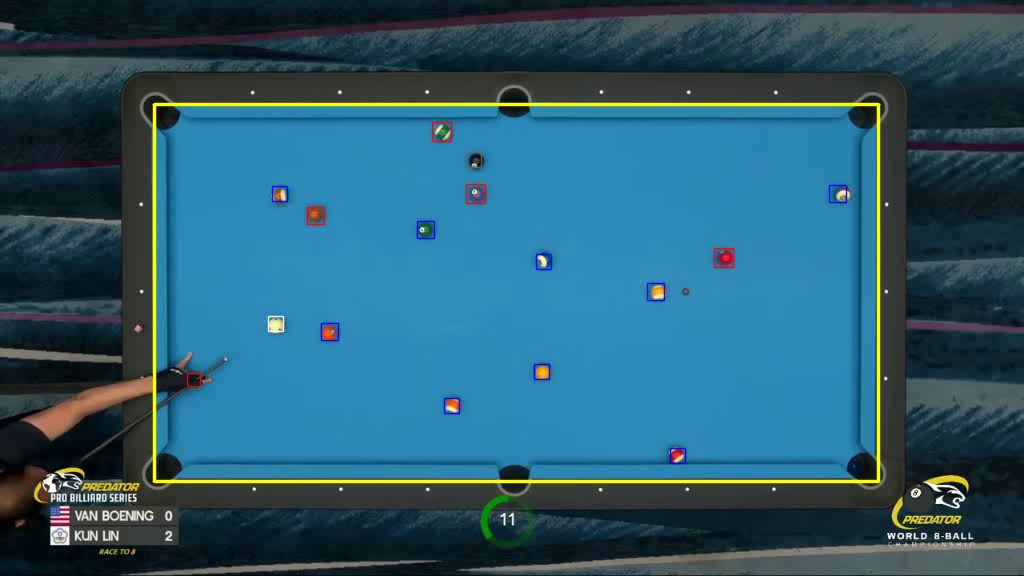
\includegraphics[width=\textwidth]{images/TableOrientation/g1_c1.jpg}
		\caption{Detection of the table and the balls with the colors representing the classes.}
		%\label{fig:game1_clip1_detection}
	\end{subfigure}
	\begin{subfigure}[b]{0.48\textwidth}
		\centering
		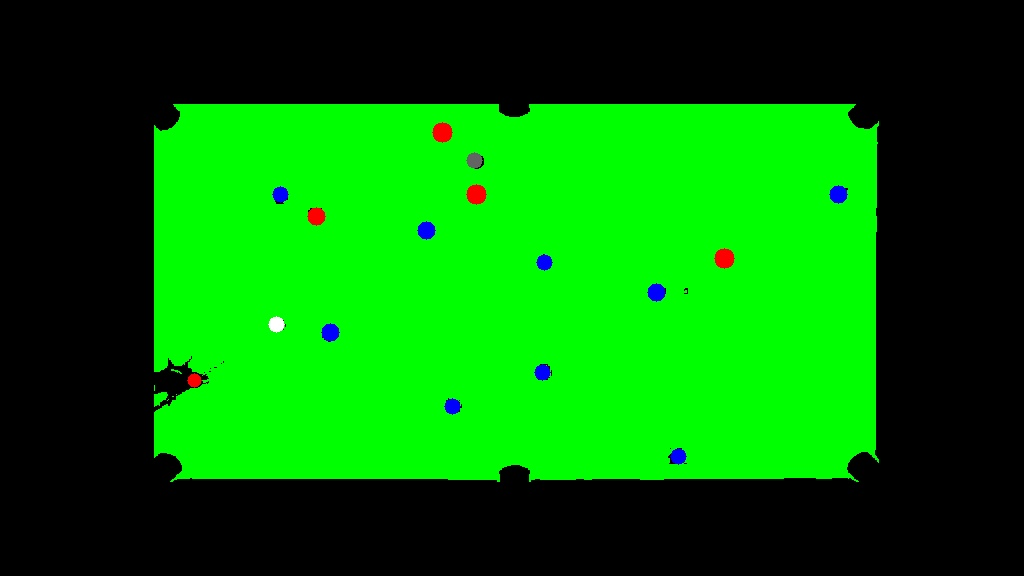
\includegraphics[width=\textwidth]{images/Segmentation/game1_clip1_segmented_balls_first_frame.jpg}
		\caption{Transformation of the table to the minimap table size}
		%\label{fig:game1_clip1_mask}
	\end{subfigure}
	\caption{game1\_clip1 first frame. The table is transformed in the wrong way because the pockets are located in the shortest edges rather than the longest ones.}
	\label{fig:game1_clip1_orientation}
\end{figure}

\begin{figure}[H]
	\centering
	\subfloat[Detection of the table and the balls with the colors representing the classes.]{
		%\label{fig:game2_clip1_detection}
		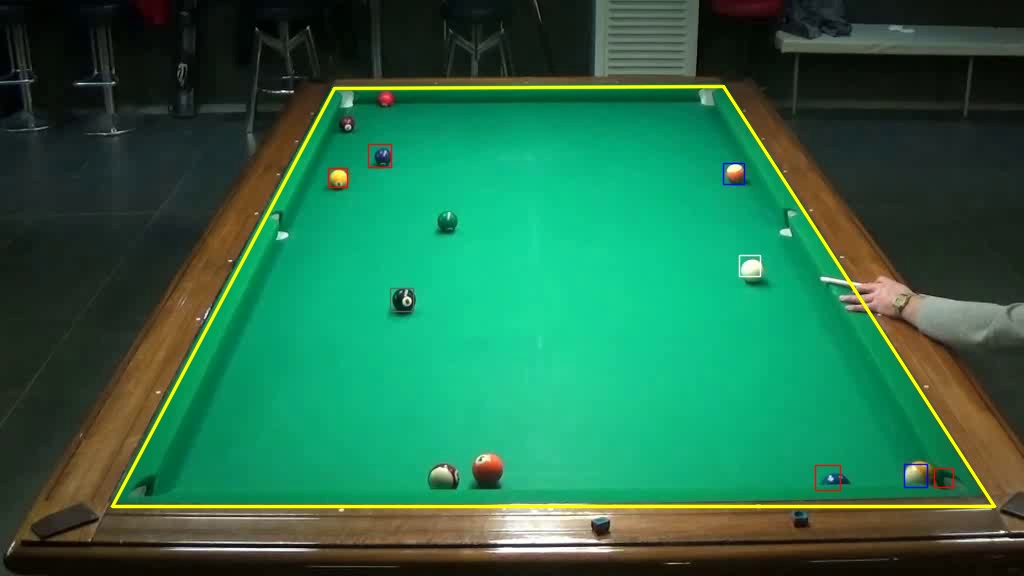
\includegraphics[width=0.48\textwidth]{images/TableOrientation/g2_c1.jpg}
	}
	\
	\subfloat[Transformation of the table to the minimap table size.]{
		%\label{fig:game2_clip1_mask}
		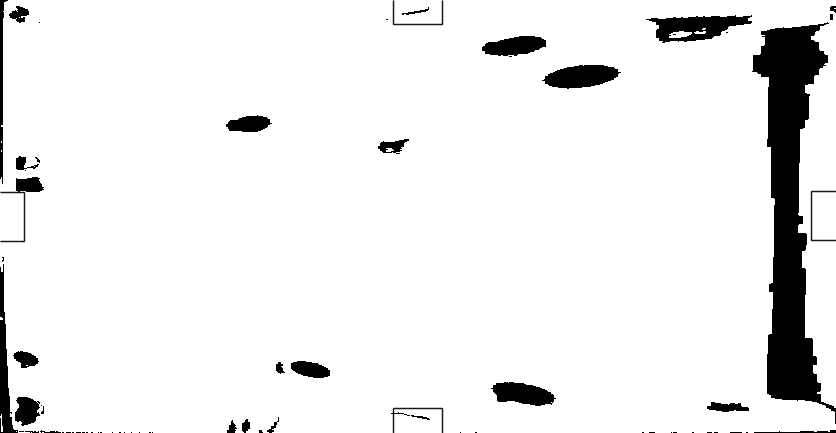
\includegraphics[width=0.48\textwidth]{images/TableOrientation/g2_c1_mask.jpg}
	}
	\caption{game2\_clip1 first frame. The table is correctly transformed. In this case, the pockets are lightly visible, but they allow the detection of the correct orientation.}
	\label{fig:game2_clip1_orientation}
\end{figure}

\begin{figure}[H]
	\centering
	\subfloat[Detection of the table and the balls with the colors representing the classes.]{
		%\label{fig:game3_clip1_detection}
		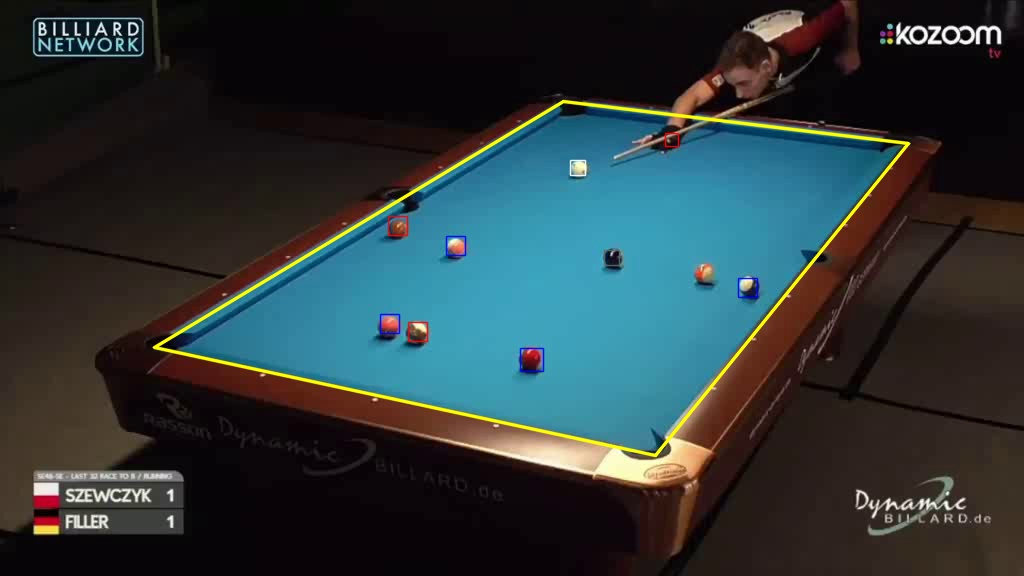
\includegraphics[width=0.48\textwidth]{images/TableOrientation/g3_c1.jpg}
	}
	\
	\subfloat[Transformation of the table to the minimap table size.]{
		%\label{fig:game3_clip1_mask}
		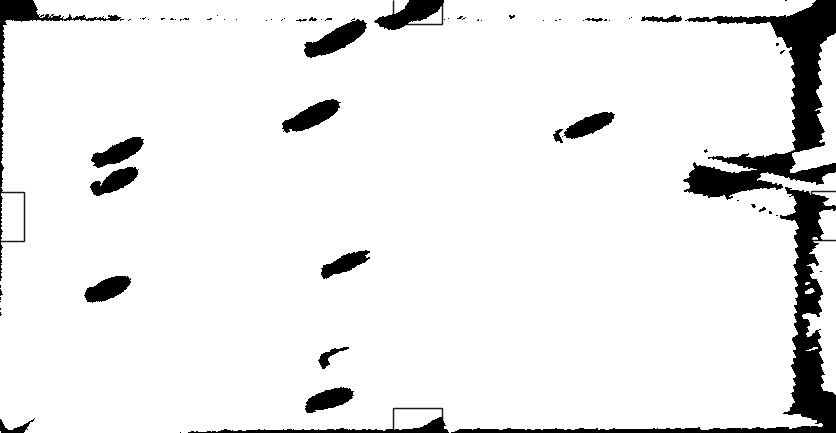
\includegraphics[width=0.48\textwidth]{images/TableOrientation/g3_c1_mask.jpg}
	}
	\caption{game3\_clip1 first frame. The table is correctly transformed. In this case, the center of one of the shortest edges has some noise due to the person playing the game; the result is correct because in the opposite edge there is no noise.}
	\label{fig:game3_clip1_orientation}
\end{figure}

\begin{figure}[H]
	\centering
	\subfloat[Detection of the table and the balls with the colors representing the classes.]{
		%\label{fig:game4_clip1_detection}
		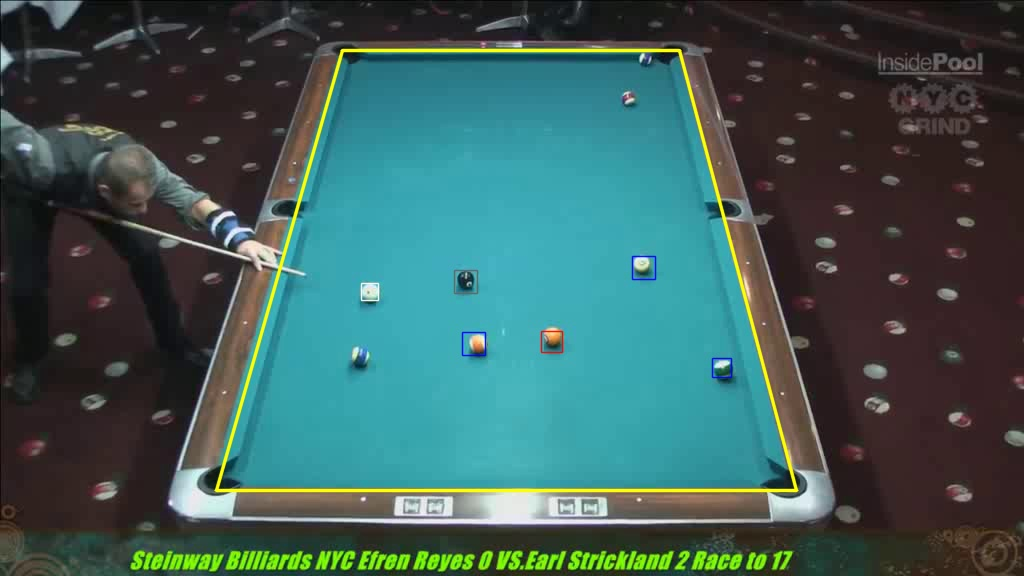
\includegraphics[width=0.48\textwidth]{images/TableOrientation/g4_c1.jpg}
	}
	\
	\subfloat[Transformation of the table to the minimap table size.]{
		%\label{fig:game4_clip1_mask}
		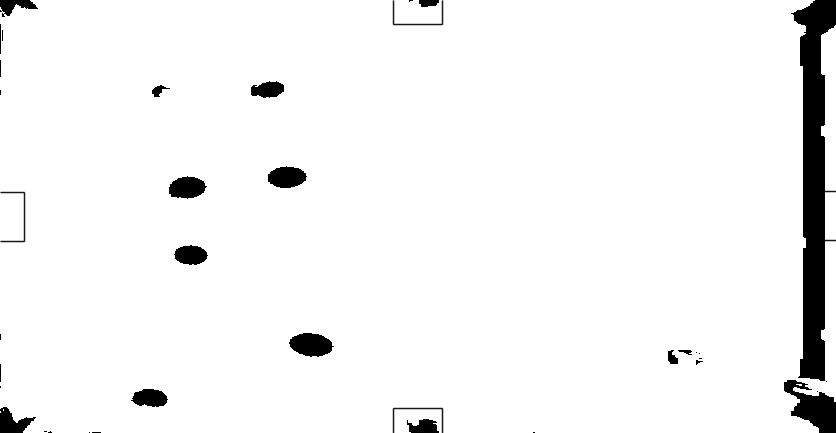
\includegraphics[width=0.48\textwidth]{images/TableOrientation/g4_c1_mask.jpg}
	}
	\caption{game4\_clip1 first frame. The table is correctly transformed. In this case, the center of one of the shortest edges has some noise due to the light of the table; the result is correct because in the opposite edge there is no noise.}
	\label{fig:game4_clip1_orientation}
\end{figure}


\subsubsection{Draw the minimap with tracking lines and balls}
Given the transformation matrix and the ball positions in the frame, it is possible to compute the positions of the balls in the minimap. This computation has been done in the \texttt{drawMinimap} method. Every time this method is called, the ball positions and the positions of the balls in the previous frame (if they have been computed by the tracker) are computed by using the

\noindent\texttt{perspectiveTransform} method. For each ball in the frame, a line between the previous position and the current position is drawn on the minimap image, passed as a parameter by reference such that all the tracking lines are kept in a single image (Figure \ref{fig:game2_clip1_tracking}). Then this image is cloned into a copy, and the current balls are drawn on it. This image is then returned (Figure \ref{fig:game2_clip1_balls}). This implementation idea comes from Alberto.

\begin{figure}[H]
	\centering
	\begin{subfigure}[b]{0.48\textwidth}
		\centering
		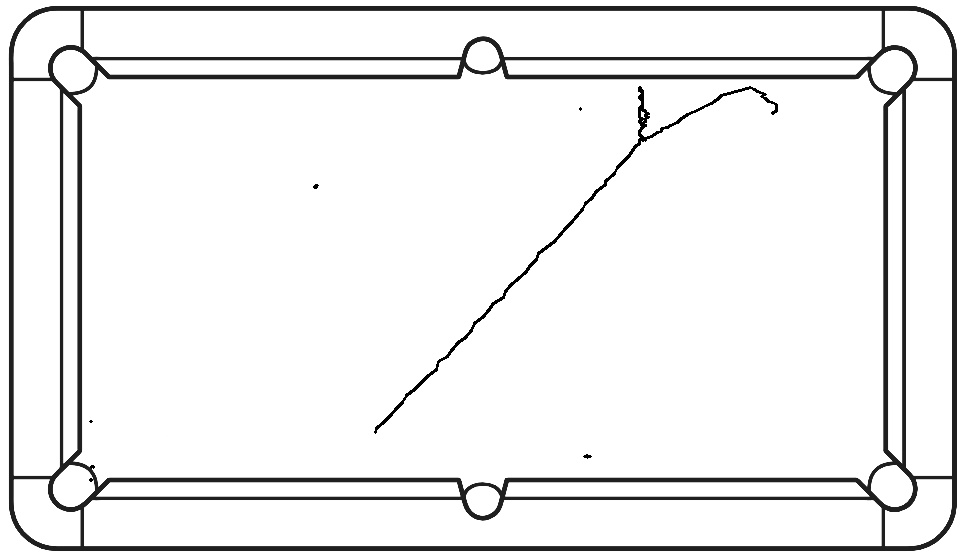
\includegraphics[width=\textwidth]{images/Minimap/g2_c1minimap_with_track.jpg}
		\caption{Minimap with tracking lines}
		\label{fig:game2_clip1_tracking}
	\end{subfigure}
	\begin{subfigure}[b]{0.48\textwidth}
		\centering
		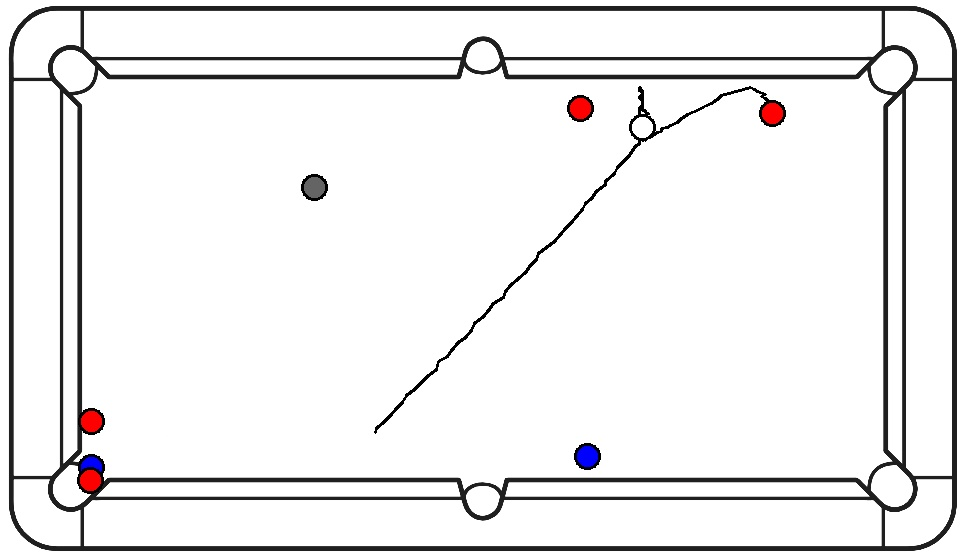
\includegraphics[width=\textwidth]{images/Minimap/g2_c1_minimap_with_balls.jpg}
		\caption{Minimap with tracking lines and balls}
		\label{fig:game2_clip1_balls}
	\end{subfigure}
	\caption{game2\_clip1. Minimap of the last frame.}
	\label{fig:game2_clip1_balls_and_tracking}
\end{figure}

The implementation and the ideas of using \texttt{getPerspectiveTransform} and

\noindent\texttt{perspectiveTransform}, and how to check the orientation of the table were from Michela.

\subsection{Video creation}
To create the output video we take the minimap and the current frame and Michele decide to do as follows:
At the beginning the function compute two values: the scaling factor for the minimap and the offset
(the first row where the minimap is placed). For the scaling factor Michele thought that
the minimap should have 0.3 of the total columns of the frame, so the scaling factor is computed as follows:
\begin{equation}
	%\text{scaling\_factor} = \frac{0.3 \times \text{frame.cols}}{\text{minimap\_with\_balls.cols}}
\end{equation}
Instead for the offset, Michele thought that the minimap should be placed at the bottom right of the frame
and it must be attached to the bottom border so first a factor is computed as follows:
\begin{equation}
	%\text{percentage} = \frac{(\text{frame.rows} - \text{scaling\_factor} \times \text{minimap\_with\_balls.rows})}{\text{frame.rows}}
\end{equation}
Then the offset is computed as follows:
\begin{equation}
	%\text{offset} = \text{percentage} \times \text{frame.rows}
\end{equation}
After that the minimap is resized and placed in bottom right corner of the output frame that
is saved in the output video.
To avoid creating the output video file and then run in some exception resulting in a not readable file,
Alberto thought about using a temporary file and then rename it to the output file only at the end where
it is sure that the file is readable.



\section{Results}

Table detection exhibits very high accuracy, in particular for each initial frame of each video four corner points are consistently identified across the dataset, the assumption that we made is that the camera does not move during a single clip so once the table is detected in the first frame we can use that information for all the frames of the same video.
In contrast, ball detection is influenced by k-means clustering. To achieve consistent and satisfactory results, a fixed random seed is incorporated into the code. This method results in an average mAP of 0.51 for the dataset.

\subsection{Quantitative results}
By executing the code in \textit{computePerformance}, the performance of the detection and segmentation are computed.
\begin{table}
	\centering
    \begin{tabular}{|c|c|}
        \hline
        mAP & mIoU \\
        \hline
        0.51 & 0.69 \\
        \hline
    \end{tabular}
    \caption{Performance of the detection and segmentation}
    \label{tab: performance}
\end{table}

\subsection{Qualitative results}
Below some qualitative results are presented.
\begin{figure}
    \centering
    \begin{subfigure}[b]{0.45\textwidth}
        \centering
        \includegraphics[width=\textwidth]{images/Detection/game1_clip1_detected_first_frame.png}
        \caption{Detection game1 clip1 first frame}
        \label{fig: game1_clip1_first_frame_detected}
    \end{subfigure}
    \begin{subfigure}[b]{0.45\textwidth}
        \centering
        \includegraphics[width=\textwidth]{images/Segementation/game1_clip1_first_frame.png}
        \caption{Segmentation game1 clip1 first frame}
		\label{fig: game1_clip1_first_frame_segmented}
    \end{subfigure}
	\caption{game1 clip1 first frame}
\end{figure}


\begin{figure}
    \centering
    \begin{subfigure}[b]{0.45\textwidth}
        \centering
        \includegraphics[width=\textwidth]{images/Detection/game2_clip1_detected_first_frame.png}
        \caption{Detection game2 clip1 first frame}
        \label{fig: game2_clip1_first_frame_detected}
    \end{subfigure}
    \begin{subfigure}[b]{0.45\textwidth}
        \centering
        \includegraphics[width=\textwidth]{images/Segementation/game2_clip1_first_frame.png}
        \caption{Segmentation game2 clip1 first frame}
		\label{fig: game2_clip1_first_frame_segmented}
    \end{subfigure}
	\caption{game2 clip1 first frame}
\end{figure}

\begin{figure}
    \centering
    \begin{subfigure}[b]{0.45\textwidth}
        \centering
        \includegraphics[width=\textwidth]{images/Detection/game3_clip1_detected_first_frame.png}
        \caption{Detection game3 clip1 first frame}
        \label{fig: game3_clip1_first_frame_detected}
    \end{subfigure}
    \begin{subfigure}[b]{0.45\textwidth}
        \centering
        \includegraphics[width=\textwidth]{images/Segementation/game3_clip1_first_frame.png}
        \caption{Segmentation game3 clip1 first frame}
		\label{fig: game3_clip1_first_frame_segmented}
    \end{subfigure}
	\caption{game3 clip1 first frame}
\end{figure}

\begin{figure}
    \centering
    \begin{subfigure}[b]{0.45\textwidth}
        \centering
        \includegraphics[width=\textwidth]{images/Detection/game4_clip1_detected_first_frame.png}
        \caption{Detection game4 clip1 first frame}
        \label{fig: game4_clip1_first_frame_detected}
    \end{subfigure}
    \begin{subfigure}[b]{0.45\textwidth}
        \centering
        \includegraphics[width=\textwidth]{images/Segementation/game4_clip1_first_frame.png}
        \caption{Segmentation game4 clip1 first frame}
		\label{fig: game4_clip1_first_frame_segmented}
    \end{subfigure}
	\caption{game4 clip1 first frame}
\end{figure}


\section{Conclusions}
Our program demonstrates consistent performance across the dataset. Notably, table detection achieves high accuracy. However, ball classification presents some challenges due to their varying sizes and colors that can sometimes are similar to the one of the table.


\end{document}
